\documentclass[a4paper]{article}
\usepackage[utf8]{inputenc}
\usepackage[T1]{fontenc}
\usepackage[french]{babel}
\usepackage{geometry}
\geometry{hmargin=3.5cm,vmargin=3.5cm}
\usepackage{graphicx}
\usepackage[nottoc, notlof, notlot]{tocbibind}

%% \usepackage[vlined, lined, linesnumbered, boxruled, french]{algorithm2e}
\usepackage{fancyhdr}
\pagestyle{fancy}

\lhead{Background}
\rhead{Simulateur de caches multi-c\oe ur}
\lfoot{ENSEIRB-MATMECA}
\rfoot{PFA 2013-2014}

\begin{document}

\thispagestyle{empty}

\vspace{\stretch{1}}
\hrule
\begin{flushleft}
\huge{Simulateur de caches sur\\architecture multi-c\oe ur :}\\
\end{flushleft}
\begin{flushright}
\Huge\textbf{Rapport}\\
\end{flushright}
\hrule

\vspace{\stretch{1}}
\noindent\textbf{Auteurs :}
\emph{DUBOIS Nicolas, GOUDET Pierre, HENG Nicolas, HONORAT Alexandre, MARAIT Gilles, PICHON Grégoire}\\
\\
\noindent\textbf{Client :}
\emph{M. BARTHOU Denis}\\
\\
\noindent\textbf{Responsable pédagogique :}
\emph{M. MORANDAT Floréal} 

\vspace{\stretch{1}}
\normalsize
\begin{center}
  Deuxième année, filière informatique\\
  Date : \today\\
  \textsc{Enseirb-Matmeca}
\end{center}


\newpage
\tableofcontents

\newpage
\section*{Introduction}

\indent Dernièrement la vitesse des processeurs a considérablement augmenté (loi de Moore) alors que le temps d'accès à la mémoire RAM (Random-Access Memory) est resté globalement le même. Pour permettre d'accèder rapidement à des éléments mémoire non contenus dans les registres, des caches sont utilisés. Cette organisation hiérarchique de la mémoire a plusieurs objectifs: \\
\begin{itemize}
\item \^Etre assez conséquente en termes de taille pour pouvoir contenu la totalité de l'espace adressable.
\item \^Etre organisée de manière à être rapide.
\item Ne pas coûter trop cher. \\
\end{itemize}

\indent Les caches permettent de stocker la mémoire utilisée récemment dans les registres, en se basant sur deux concepts: la localité spatiale et la localité temporelle. La localité temporelle stipule qu'une cellule mémoire accédée récemment sera très probablement utilisée dans un futur proche. La localité spatiale est l'idée que si l'on accède à une cellule mémoire $X$, la cellule mémoire $X+1$ a de grandes chances d'être utilisée. \\

\indent Les mémoires de haut niveau, proches du processeur, sont généralement de petite taille. Leur coût est conséquent mais leur accès est très rapide. On peut résumer comme suit une hiérarchie mémoire classique: \\

\begin{figure}[!h]
\begin{center}
   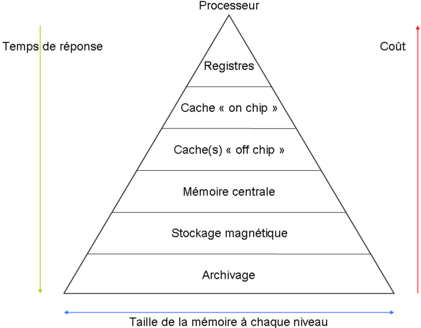
\includegraphics[scale=0.75]{hierarchy.png}
   \caption{\label{hierarchy} Hiérachie mémoire}
\end{center}
\end{figure}

\indent De cette manière, quand le processeur utilise une donnée qui est dans le cache, il fait un Hit: il n'a pas besoin de la charger à partir de la mémoire principale. Lorsque la donnée dont il a besoin n'est pas présente dans le cache, il fait un Miss et le coût d'accès à la donnée est beaucoup plus important. \\

\indent Le but de ce document est de résumer un certain nombre de techniques relatives à la bonne gestion de cette hiérarchie, en se focalisant sur les caches. Nous commencerons par expliciter le comportement d'un cache en général, avant d'étudier les moyens mis en {\oe}uvre afin d'assurer la cohérence de l'ensemble des caches. Nous finirons par proposer quelques algorithmes permettant de simuler de manière la plus générique possible le comportement des caches.

\newpage
\section{Fonctionnement d'un cache}
\indent Cette partie entend préciser le fonctionnement général d'un cache: comment il est possible d'y ajouter une donnée, quelle est la correspondance entre les blocs mémoires et les lignes de cache ou encore comment une donnée peut être evincée d'un cache.

\subsection{\'Etiquettes}
\indent Quand un bloc mémoire (généralement $1$ octet) est ajouté dans le cache, la ligne entière correspondante ($32$ ou $64$ octets) est chargée dans le cache, afin d'exploiter le principe de localité spatiale et de faire du prefetching de données. Pour pouvoir retrouver une donnée dans le cache, une table d'étiquettes est tenue à jour. Concrètement, une adresse mémoire est séparée en trois champs comme sur la figure suivante: \\

\begin{figure}[!h]
\begin{center}
   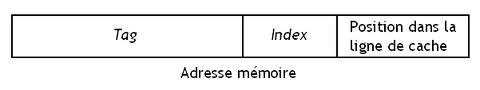
\includegraphics[scale=0.50]{etiquette.jpeg}
   \caption{\label{etiquette} Adresse mémoire}
\end{center}
\end{figure}

\indent Le tag est stocké dans la table des étiquettes, il servira a identifier les différents blocs mémoires pouvant être au même endroit dans un cache. L'index correspond au numéro de set dans lequel se trouve la ligne de cache. Pour finir l'offset correspond au bloc dans la ligne de cache.

\subsection{Fonction de correspondance}
\indent Un cache de taille $n$ contient un ensemble $p$ de lignes de taille $m$, tels que $n = p \times m$. Afin de placer et récupérer une donnée dans le cache, une fonction de correspondance avec la mémoire est nécessaire. Il existe trois cas de figure. Pour la suite, nous prendrons: \\
\begin{itemize}
\item $i$ le numéro de set du cache
\item $j$ le numéro du bloc mémoire
\item $s$ le nombre de sets du cache
\item $k$ l'associativité du cache 
\end{itemize}

\subsubsection{Direct associative}
\indent Un cache est en correspondance directe si à chaque bloc mémoire est associé une unique ligne du cache. Le nombre de sets, $s$, du cache est alors égal à son nombre de lignes, $p$. Lorsqu'un bloc mémoire $j$ est ajouté dans le cache, la ligne correpondante est chargée à la ligne $i = j\ modulo\ s$. Avec ce type de cache, il est facile d'ajouter ou de retrouver une données. Cependant, si plusieurs blocs mémoires correpondant à la même ligne de cache sont fréquemment utilisés, il faudra sans cesse supprimer et ajouter des données dans le cache.

\subsubsection{Fully associative}
\indent Un cache est en correspondance associative si chaque bloc mémoire peut être mis dans n'importe quelle ligne du cache. Il n'y a alors qu'un seul set. L'inconvénient précédent n'est plus existant, cependant il devient beaucoup plus compliqué de rechercher une donnée dans le cache. L'ensemble des tags doit en effet être parcouru.

\subsubsection{$k$-ways associative}
\indent Les deux cas présentés précedemment présentent des inconvénients. Généralement, un cache profite des avantages des deux visions en faisant un compromis. Dans le cas de la correspondance associative par ensemble, chaque set possède un nombre $k$ de lignes, appelé associativité du cache et tel que $p=k \times s$. La fonction de correspondance est telle que $i = j\ modulo\ s$. De cette manière, un bloc mémoire peut se trouver dans un ensemble de $k$ lignes. Il est donc possible d'avoir plusieurs blocs mémoires correspondant au même ensemble sans trop perdre en performances et l'algorithme de recherche est plus efficace que dans le cas de la correspondance associative.

\begin{figure}[!h]
\begin{center}
   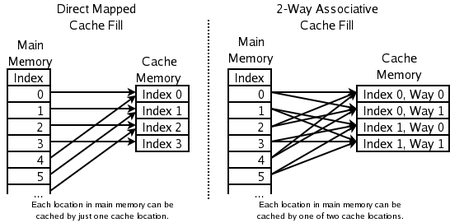
\includegraphics[scale=0.60]{associative.png}
   \caption{\label{associative} Fonction de correspondance}
\end{center}
\end{figure}

\subsection{Politiques de remplacement}
\indent Lorsque l'on souhaite ajouter une ligne dans un set plein, il faut au préalable evincer une ligne de ce set. Pour cela, il existe différentes méthodes:

\paragraph{FIFO.} La première solution consiste à supprimer la ligne la plus ancienne du cache. Cela correspond à la formule: ``First In, First Out''.

\paragraph{LFU.} Une autre solution consiste à supprimer la ligne qui a été le moins utilisée: ``Least Frequently Used''. Pour cela, chaque ligne de cache possède un compteur qui sera incrémenté à chaque utilisation de la ligne. 

\paragraph{LRU.} La dernière solution, généralement utilisée, consiste à favoriser le principe de localité temporelle en supprimant la ligne du set qui a la plus ancienne date d'utilisation: ``Least Recently Used''.

\newpage
\section{Gestion de la cohérence}
\indent Dans les systèmes actuels, un processeur n'est plus composé d'un unique c{\oe}ur, mais de plusieurs. Chaque c{\oe}ur possède généralement deux caches de plus haut niveau: le L1i pour stocker les instructions et le L1d pour stocker les données. Si les interactions entre ces deux caches sont minimes, il est difficile de mélanger instructions et données, la cohérence entre les différents c{\oe}ur est un problème de taille.

\subsection{Présentation du problème}
\indent Les caches sont utilisés à chaque load/store. Si il est possible que plusieurs caches possèdent la même donnée et la lisent en même temps, il est primordial de définir un protocole de cohérence afin qu'une donnée ne puisse pas être modifiée simultanément dans deux caches. Pour cela, des techniques hardwares sont mises en place afin de définir qui a la priorité si deux c{\oe}urs veulent modifier une même donnée. \\

\indent Par ailleurs, un protocole de cohérence est mis en {\oe}uvre à chaque load/store afin que les différents caches soit informés des modifications les concernant et que la consistance du système soit assurée. Ce protocole est propre à un niveau de cache. Dans un cas classique, il y aura un protocole de cohérence entre les L1 et entre les L2.

\subsection{Protocoles de cohérence}
\indent Nous étudierons uniquement le protocole de type MSI et ses dérivés: MESI, MOSI et MOESI. Chaque ligne de cache possède un état qui permet de gérer la cohérence. Les différents états sont: \\
\begin{itemize}
\item M: Une ligne est dans l'état modifié si c'est la seule copie valide dans l'ensemble des caches du niveau. Dans ce cas, si la ligne est evincée du cache, elle doit être recopiée en mémoire, via un write back. \\
\item S: Une ligne est dans l'état shared si elle est valide et qu'elle n'a pas été modifiée. Dans ce cas, plusieurs caches peuvent possèder la ligne. \\
\item I: L'état invalide est utilisé pour une ligne qui n'est pas valide. Le contenu de la ligne n'est pas viable, il ne faut pas l'utiliser. \\
\item E: Une ligne est dite exclusive si c'est, dans le niveau, la seule copie valide. Une ligne dans cet état n'a pas été modifiée et les données de la ligne sont identiques à celles de la mémoire principale. \\
\item O: L'état owned est utilisé pour un cache qui possède une donnée invalide dans la mémoire principale. Plusieurs caches peuvent possèder la même donnée, ils seront alors dans l'état S. \\
\end{itemize}

\indent L'état M est utilisée lorsque la donnée a été modifiée par un c{\oe}ur. Il existe deux cas de propagation des modifications. Dans le choix de la politique Write-Through, la donnée est directement recopiée dans la mémoire principale pour éviter de futurs problèmes de cohérence. Dans le cas de la politique Write-Back, la donnée est modifiée uniquement dans le cache. Les autres caches et la mémoire principale peuvent savoir que la donnée a été modifiée, en revanche ils n'ont pas la dernière copie valide. Ils peuvent l'obtenir lors des Write-Backs: lorsque la donnée est evincée du cache ou lorsqu'elle est demandée à un plus haut niveau pour des soucis de cohérence.

\newpage
\indent Le protocole de cohérence le plus utilisé est MESI. Voici certaines caractéristiques de ce protocole: \\
\begin{itemize}
\item Lorsqu'un cache charge une donnée, il demande si un autre cache possède la donnée. Si un cache possède la donnée dans l'état M, alors ce cache fait un Write-Back et invalide sa donnée. Si un autre cache possède la donnée en état E, la donnée passe dans l'état S pour les deux caches. Si plusieurs (ou un seul) caches possèdent la donnée dans l'état S, la donnée est ajouté dans l'état S.
\item Si un cache possède une donnée dans l'état M ou E et fait un nouveau store sur la ligne de cache, son état devient M et aucune information n'est transmise aux autres caches.
\item Si un cache fait un store sur une donnée dans l'état S, la même donnée située dans les autres caches est invalidée. \\
\end{itemize}

\indent Voici l'automate du protocole: \\

\begin{figure}[!h]
\begin{center}
   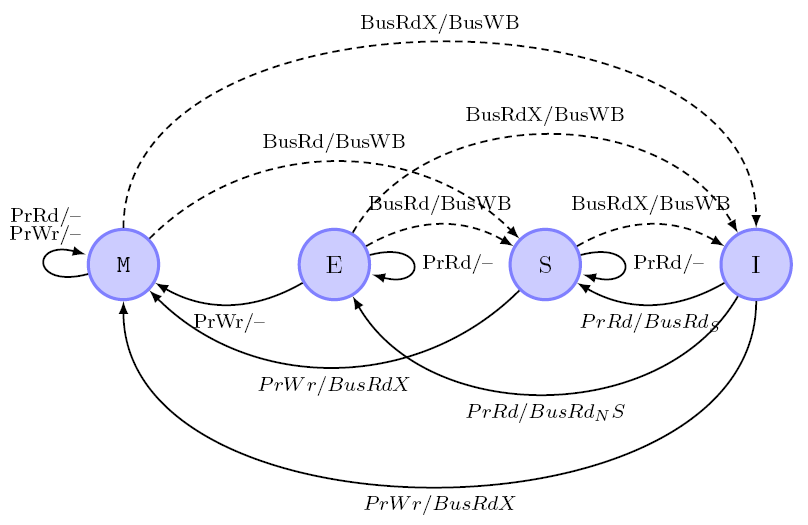
\includegraphics[scale=0.45]{mesi.png}
   \caption{\label{mesi} Automate du protocole MESI}
\end{center}
\end{figure}

\indent Pour l'état O, la différence est que les interactions avec la mémoire principale sont moins importantes. En effet, lorsqu'un cache qui n'a pas la donnée fait un load, le cache possédant la donnée dans l'état O peut lui donner sans faire de Write-Back. Cela permet de garder plus longtemps la donnée modifiée.

\newpage
\section{Fonctionnement global}

\subsection{Caches inclusifs}

\subsection{Caches exclusifs}

\subsection{Caches non-inclusifs}


\newpage
\section{Comportements spéciaux}

\subsection{Utilisation d'un victim cache}
\indent Généralement, des caches à $k$ voies associatifs sont utilisés, car la fonction de recherche d'une donnée est peut coûteuse et plusieurs blocs mémoire correspondant à une même place peuvent être stocké dans un cache. Dans la plupart des cas, le nombre de voies varie entr e $2$ et $12$. \\

\indent Dans certains cas, il est possible que le nombre de voies ne soit pas suffisant car un ensemble de blocs mémoire correspondant au même set est très utilisé. Cela est notamment vrai pour les L1 qui possèdent généralement peu de voies. Pour palier ce problème et limiter les échanges de données entre les L1 et les L2, il est possible d'utiliser un buffer pour stocker les victimes d'éviction. Ce buffer est de petite taille, par exemple $8$ fois la taille d'une ligne de cache. \\

\indent De cette manière, lorsqu'un donnée est supprimée du L1, elle est placée dans le buffer correspondant. Lorsque le L1 fait un Miss, il commence par regarder dans le buffer (le coût est alors faible étant donné la taille du buffer) avant de regarder dans le L2. Cette idée permet donc de palier de façon peut coûteuse au problème d'un set qui n'aurait pas assez de voies.

\subsection{Tracking}
\subsubsection{Supprimer les données}
\indent Lorsqu'un cache L1 utilise une donnée qu'il possède déjà dans son cache, les flags utilisés par les politiques de remplacement sont mis à jour afin de supprimer les bonnes données lorsqu'un set sera plein. Cependant, les caches de plus haut niveau (L2, L3) ne sont pas mis au courant que la donnée a été utilisée et ils ne changent donc pas les flags de remplacement. Ainsi, lorsque le L2 aura un set plein, il se peut qu'il supprime une donnée très utilisée dans un L1. \\

\indent Dans le cas d'un cache inclusif, il faut donc, à la suppression d'une donnée, invalider la donnée dans les caches en dessous afin de conserver le caractère inclusif. Pour limiter ce problème, les L2 et les L3 peuvent suivre les données, c'est-à-dire posséder une table indiquant quels caches de niveau plus bas ont également la donnée. De cette manière, les politiques de remplacement peuvent être adaptées en définissant des priorités: par exemple, éviter de supprimer les données qui sont contenues dans beaucoup de caches.

\subsubsection{Savoir qui a les données}
\indent cf NUCA

\newpage
\section{Algorithmes de simulation}

\subsection{Interaction entre les différents niveaux de caches}

\subsection{Gestion des différentes modularités}

\newpage
\nocite{*}
\bibliographystyle{plain}
\bibliography{rapport}

\end{document}
